\documentclass[12pt]{article}
\usepackage{amsmath}
\usepackage{listings}
\usepackage{xcolor}
\usepackage{float}

\definecolor{codegreen}{rgb}{0,0.6,0}
\definecolor{codegray}{RGB}{4,118,219}
\definecolor{codepurple}{rgb}{0.58,0,0.82}
\definecolor{backcolour}{RGB}{0,27,51}
\definecolor{textcolour}{RGB}{38, 149, 245}

\lstdefinestyle{mystyle}{
    backgroundcolor=\color{backcolour},   
    commentstyle=\color{codegreen},
    keywordstyle=\color{magenta},
    numberstyle=\tiny\color{codegray},
    stringstyle=\color{codepurple},
    basicstyle=\ttfamily\color{textcolour}\footnotesize,
    breakatwhitespace=false,         
    breaklines=true,                 
    captionpos=b,                    
    keepspaces=false,                 
    numbers=left,                    
    numbersep=5pt,                  
    showspaces=false,                
    showstringspaces=false,
    showtabs=false,                  
    tabsize=2
}

\lstset{style=mystyle}

    \title{\textbf{Projektarbeit}}
    \author{Jan Philipp Fortowski}
    \date{02.10.2023}
    
    \addtolength{\topmargin}{-3cm}
    \addtolength{\textheight}{3cm}
\usepackage{graphicx}
\begin{document}

\maketitle
\tableofcontents
\thispagestyle{empty}

\section{Das Netzwerk}
\subsection{Initialisierung}
\subsubsection{Grundgedanke}
Bei der Initialisierung des Netzwerkes soll eine Instanz der Klasse NeuralNetwork erstellt werden. Wichtig ist hierbei, dass das Netzwerk über alle Variablen verfügt, die hierbei wichtig sind, und dass es im Konstruktor möglich ist, wichtige Eigenschaften so dynamisch anzulegen, wie es nur geht. Für den Learn Algorithmus ist später eine LearnRate wichtig, das wird später im Backpropagation Algorithmus wichtig. Abgesehen davon, muss es möglich sein, die Menge der versteckten Schichten, sowie die Menge der Nodes auf diesen festzulegen. für eine leichtere Lesbarkeit, und leichtere Skalierung des Netzwerks, ist es Vorteilhaft, die Schichten, oder auch Layer, in einer eigenen Klasse festzulegen.

Diese Layer müssen also auch vorbereitet werden. Wie bereits erwähnt, ist jede Schicht durch Kanten mit der nächsten Schicht verbunden.  Von jedem Knoten aus dem Input Layer gehen Kanten an jeweils jeden Knoten der ersten versteckten Schicht. Und genau so ist es zwischen der Versteckten Schicht zu jeder nachfolgenden versteckten Schicht, bis hin zum Output Layer. Jede diese Kanten ist gewichtet, und diese gewichte müssen in jedem Layer gespeichert werden. Das Input Layer ist mehr Symbolisch dargestellt, da es sich bei den Knoten dieser Schicht nur um die Inputs handelt, mit denen das Netzwerk gefüttert werden soll. Bezogen auf den MNIST Datensatz, bedeutet das, dass jeder Pixel eines Bildes ein Knoten der Input Layer ist. Daraus ergibt sich bei 28 X 28 Pixeln eine Input Schicht von 784 Knoten. Diese unterliegen natürlich noch keine Activation Function/Schwellwertfunktion, und werden daher direkt in die erste versteckte Schicht geleitet. Die Implementation dieser Schichten kann von hier an generalisiert werden.

Jede Schicht sollte alle Gewichte der Kanten speichern, mit denen sie mit der vorherigen Schicht verbunden sind. Diese Gewichte lassen sich in Form einer Matrix speichern. Die erste Dimension dieser Matrix entspricht der Anzahl der Inputs, die der Layer aus der vorherigen Schicht erhält, also die Anzahl der Outputs der vorherigen Schicht. Die Zweite Dimension entspricht der Knoten, über die das Layer verfügt.

Ein bestimmtes Gewicht kann also so notiert werden:

Die Kante von dem 3ten Knoten der Input Schicht zum 2ten Knoten der versteckten Schicht wird gewichtet durch das Gewicht \(W_{3|2}\).

Das Layer braucht, im Initialisiert zu werden, also lediglich zwei Werte, die Anzahl der Input Nodes, und die Anzahl der eigenen Output Nodes. Daraus kann ein 2-dimensionales Array erstellt werden, mit eben diesen Abmaßen. An dieser Stelle muss darauf hingewiesen werden, dass es Sinnvoll ist, die Matrix von vornherein transponiert zu speichern, da es für die meisten Rechnungen Notwendig sein wird, diese ohnehin zu Transponieren.

\subsubsection{Code}
Das Neuronale Netzwerk braucht zuerst ein Array, in welchem alle Layer gespeichert sind, außerdem ein Double für die LearnRate.

Der Konstruktor hat zunächst die Parameter für die learnRate, und dann noch "variable arguments", welche die jeweilige Anzahl an Knoten pro Schicht angeben sollen.

Wie oben erklärt, ist es nicht Notwendig, eine eigene Schicht für die Input Schicht zu instantiieren. Daher fängt die For-Schleife auch erst bei 1 an. Der erste integer, der übergeben wird, muss die Größe der Input Schicht wiedergeben, beim MNIST Datensatz also 784. Der letzte Integer gibt die Größe der Output Schicht an. Die Output Schicht muss so groß dein, wie die Menge, der möglichen Antworten. Bei dem MNIST handelt es sich um die Handschriftlichen zahlen von 0 - 9, daher muss die Output Schicht 10 Knoten haben. Alle anderen Integer, die dazwischen eingetragen werden, entsprechen der Größe einer jeden versteckten Schicht.

\begin{lstlisting}[language=Java]
public class NeuralNetwork {
    Layer[] layers;
    double learnRate;

    // Initialisierung
    public NeuralNetwork(double learnRate, int... layerSizes) {
        layers = new Layer[layerSizes.length - 1];
        for (int i = 0; i < layers.length; i++) {
            layers[i] = new Layer(layerSizes[i], layerSizes[i + 1]);
        }
        this.learnRate = learnRate;
    }
}
\end{lstlisting}

Um ein Layer zu erstellen, wird, wie oben beschrieben, die Menge der Outputs der vorherigen Schicht, und die Menge der eigenen Knoten gebraucht, damit die Gewichtsmatrix mit den richtigen Dimensionen instantiiert wird.

Bei diesem Schritt ist es wichtig, dass die Gewichte mit zufälligen Werten vor instantiiert werden. Das kann dabei helfen, dass das Netzwerk durch das Zufallsprinzip bereits näher an einem Globalen Minimum der Error Funktion startet, als an einem schlechteren Lokalen Minimum. Außerdem vermeidet man dadurch auch Symmetrie: Wenn alle gewichte mit dem gleichen Wert anfangen, ist auch die Änderungsrate meist die gleiche. Dadurch kommt es vor, dass sich die Neuronen im schlimmsten Fall auf die gleichen Merkmale konzentrieren. Die Vorbelegung dieser Arrays verlagern wir in diesem Beispiel auf eine andere Klasse, um die Hauptklassen hier leserlich zu halten. Der Gesamte Code ist im Anhang zu finden.

Die Gewichtsmatrix wird hier bereits transponiert aufgebaut.
\begin{lstlisting}[language=Java]
public class Layer {

    int numInputNodes, numOutputNodes;
    double[][] weights;

    public Layer(int numInputNodes, int numOutputNodes) {
        this.numInputNodes = numInputNodes;
        this.numOutputNodes = numOutputNodes;
        weights = NNMath.RandomDoubleArrayMatrix(numOutputNodes,numInputNodes);
    }
}
\end{lstlisting}


\subsection{Querry}
\subsubsection{Grundgedanke Querry}
Die Querry Funktion ist dazu da, um ein Ergebnis vom Netzwerk zu erlangen. Im Prinzip wollen wir ein Array, in welchem für jede Antwortmöglichkeit die Wahrscheinlichkeit zu finden ist, die das Netzwerk der jeweiligen Antwort zumisst.
Das heißt also, dass die Funktion erstmal im "NeuralNetwork" die Inputs braucht. Die Inputs müssen von Schicht zu Schicht gereicht werden, müssen in den einzelnen Knoten verarbeitet werden und dann als Output zurückgegeben werden. Die Outputs der ersten Schicht werden dann zu den Inputs für die nächste Schicht und immer so weiter bis die Output Schicht die ein Ergebnis liefert.

\subsubsection{Querry Code}
\begin{lstlisting}[language=Java]
// Abfragen in NeuralNetwork.java
    public double[] Querry(double[] inputs) {
        for (Layer layer : layers) {
            inputs = layer.CalculateOutputs(inputs);
        }
        return inputs;
    }
\end{lstlisting}

\subsubsection{Grundgedanke CalculateOutputs}
Im Layer Skript müssen die Outputs berechnet werden. Dazu können wir uns die Ursprüngliche Inspiration für neuronale Netzwerke ansehen, das Neuron!
\begin{figure}[htp]
\centering
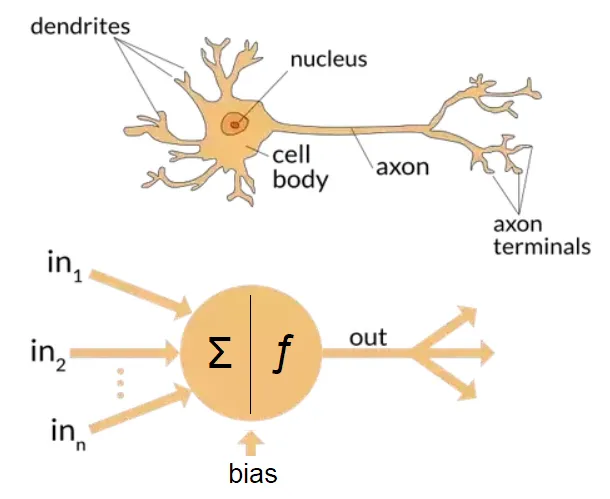
\includegraphics[scale=0.40]{/home/kater/Projekte/testlayer/NNLayers/Obsidian/Notes/Images/Pasted image 20230912175903.png}
\caption{Das Neuron}
\label{Was kommt hier rein?}
\end{figure}

Da es sich nur um eine Lose Inspiration handelt, ist es nicht notwendig, sich tiefer mit dem Gehirn auseinander zusetztes, allerdings war es tatsächlich die Inspiration für das neuronale Netzwerk. Das Gehirn besteht aus einer Vielzahl an Neuronen, Schätzungsweise aus \(10^{10}\) bis \(10^{11}\) Nervenzellen (Quelle Einführung in Neuronale Netzte Burkhard Lenze ToDo).
Wichtig sind bei dem Neuron die folgenden Bestandteile:

\begin{itemize}
    \item Dendriten
    \item der Zellkörper
    \item das Axon
\end{itemize}

Die ein Neuron hat mehrere Dendriten, die dazu verwendet werden, um Impulse aufzunehmen. Also können sie mit unseren Inputs verglichen werden. Der Zellkörper ist dafür da, die Impulse zu verarbeiten. Es wurde beobachtet, dass ein bestimmter Schwellwert überschritten werden muss, damit ein Neuron selbst wider einen Impuls abgibt. Dies werden wir mit einer Aktivierungsfunktion ebenfalls simulieren, doch dazu später mehr. zuletzt hat jedes Neuron ein Axon, welches dazu verwendet wird, um einen Impuls abzugeben. Daher ist es mit den Outputs eines Knotens vergleichbar.
Genau wie bei dem Neuron, wird in dem Neuronalen Netz zuerst jeder Input in jeden Knoten geleitet, dort dann verarbeitet, und die Ergebnisse dieser Verarbeitung werden an die nächste Schicht weitergeleitet.

\subsubsection{Berechnung Der Outputs}
Sehen wir uns zunächst ein Einfaches Netzwerk mit einer versteckten Schicht an. Jede Schicht hat nur einen Knoten:
\begin{figure}[htp]
\centering
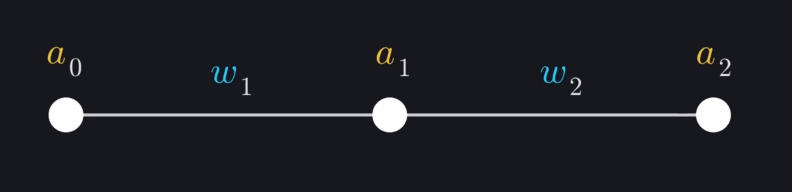
\includegraphics[scale=0.50]{/home/kater/Projekte/testlayer/NNLayers/Obsidian/Notes/Images/Pasted image 20230912184748.png}
\caption{Ein simplifiziertes Netzwerk}
\label{Was kommt hier rein?}
\end{figure}

Der erste Knoten wird \(a_0\) genannt, und entspricht schlichtweg dem Input. Dieser wird an die erste Schicht geleitet, an alle darin vorhandenen Knoten. Dort wird es erst gewichtet, das heißt mit dem Gewicht \(w_1\), welches der Kante zugewiesen ist multipliziert. Hier wird es jetzt Spannend. Nachdem alle Inputs in unseren Knoten miteinander verrechnet sind, muss das Ergebnis erst noch durch die Aktivierungsfunktion.

\subsubsection{Aktivierungsfunktion}
Die am Häufigsten genutze Aktivierungsfunktion ist die Sigmoid Funktion. Diese sieht so aus:
\[
\sigma (x) = \frac{ 1 }{ (1+e^{ -x }) }
\]

\begin{figure}[htp]
\centering
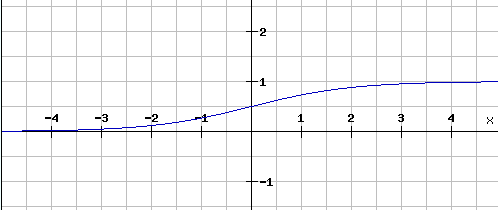
\includegraphics[scale=0.70]{/home/kater/Projekte/testlayer/NNLayers/Obsidian/Notes/Images/Pasted image 20230912192401.png}
\caption{Sigmoid Funktion}
\label{Was kommt hier rein?}
\end{figure}

Jeder Wert, der hier hinein läuft, wird auf einen Wert zwischen 0 und 1 verkleinert. 
Um ein Starkes Signal an die Nächsten Schicht zu senden, muss die Summer aller eingegangenen und danach gewichteten Signale Groß genug sein, um nach der Sigmoid Funktion noch näher an der 1 zu sein als an der 0. 
Es gibt eine ganze Reihe dieser Funktionen, hier einige Beispiele mit Erklärung:
\\\\


\begin{figure}[H]
\textbf{Die Identität}\\\\
\centering
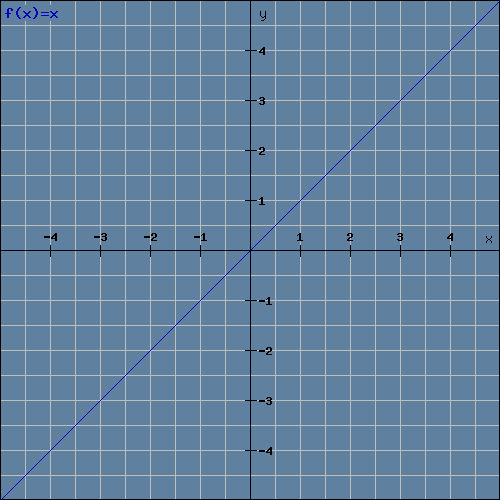
\includegraphics[scale=0.60]{/home/kater/Projekte/testlayer/NNLayers/Obsidian/Notes/Images/Pasted image 20230912194736.png}
\caption{Die Identität}
\label{Was kommt hier rein?}

Hierbei ist \emph{f(x) = x} Die Werte können dabei allerdings zu Groß werden, und daher benutzt man lieber die Sigmoid Funktion.

\end{figure}


\begin{figure}[H]
\textbf{Die Sprung Funktion}\\\\
\centering
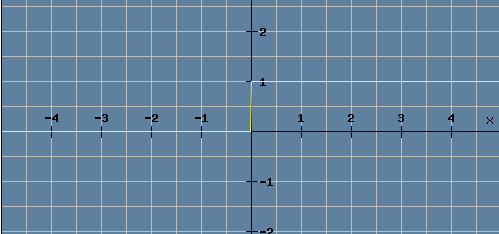
\includegraphics[scale=0.60]{/home/kater/Projekte/testlayer/NNLayers/Obsidian/Notes/Images/Pasted image 20230912195705.png}
\caption{Die Identität}
\label{Was kommt hier rein?}

Diese Funktion gibt bei \(\left\{ x>=0 \right\}\) eine 1 aus, bei \(\left\{ {x<0} \right\}\)  immer eine 0.
Dadurch können allerdings Sprunghafte veränderungen im Netztwerk eintreten, die unvorteilhaft sind.

\end{figure}

\begin{figure}[H]
\textbf{ReLu}\\\\
\centering
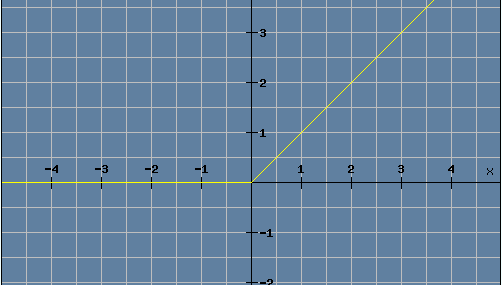
\includegraphics[scale=0.60]{/home/kater/Projekte/testlayer/NNLayers/Obsidian/Notes/Images/Pasted image 20230912200758.png}
\caption{Die Identität}
\label{Was kommt hier rein?}

Ähnlich wie \emph{Die Identität}, allerdings verläuft sie bei \(\left\{ {x<0} \right\}\) bei 0.
ReLu wird auch häufiger verwendet.

\end{figure}

Anmerkung des Autors der Arbeit: Ich habe nach einer Möglichkeit gesucht, die recht aufwendige Sigmoid Funktion etwas kosten effizienter ausrechnen zu lassen. Dabei habe ich einen Hinweis gefunden. Die Sigmoid Funktion kann im vorhinein in Hundert Schritten in eine Look Up Tabelle eingetragen werden, so dass sie nicht mehr jedes mal ausgerechnet werden muss. Dabei habe ich festgestellt, dass das Netzwerk kaum an Geschwindigkeit gewinnt, allerdings 2 bis 4\% an Genauigkeit gewinnt. Mir ist nicht vollends klar, woher diese Verbesserung kommt, allerdings sind mir derartige Beobachtungen schon häufiger untergekommen. Meist scheint es daran zu liegen, dass es dem Netzwerk schwerer fällt, sich in einem Lokalen Minimum fest zufahren. Dies ist an dieser Stelle allerdings reine Spekulation.

\subsubsection{Code zur Aktivierungsfunktion}
Den Code für die Aktivierungsfunktion. Um Die Funktionen später leichter austauschen zu können, Implementieren wir hier die Abstrakte Klasse "Activation", und implementieren dann die Unterklassen Sigmoid und ReLu. Eine Statische Methode "getActivation" ermöglicht es, aus jedem Kontext heraus auf die richtige Activation Function zuzugreifen. Mit der setter Methode kann man eine andere Activation Klasse auswählen.
\begin{lstlisting}[language=Java]
public abstract class Activation {
    public abstract double ActivationFunction(double weightedInput);

    static Activation activation = new Sigmoid();

    public static Activation geActivation(){
        return activation;
    }
    public static void setActivation(String Activation){
        switch (Activation) {
            case "Sigmoid":
                activation = new Sigmoid();
                break;
            case "ReLu":
                activation = new ReLu();
                break;
            default:
                activation = new Sigmoid();
                break;
        }
    }
}

class Sigmoid extends Activation{
    public double ActivationFunction(double weightedInput) {
        return 1.0 / (1 + Math.exp(-weightedInput));
    }
}

class ReLu extends Activation{
    public double ActivationFunction(double weightedInput) {
        return Math.max(0, weightedInput);
    }
}
\end{lstlisting}

\subsubsection{Layer Implementation}
Nach diesem Stück Vorarbeit kommen wir nun zum Abschluss der Querry. Wie genau Setzen wir das alles jetzt zusammen?
Wie bereits vorbereitet, wird jede Schicht vom NeuralNetwork in der Querry Methode aufgerufen. von jedem Layer wird die Methode "CalculateOutputs(double[] inputs)" aufgerufen, mit den Inputs versorgt, und danach werden die Outputs erwartet, um an die nächste Schicht weitergegeben zu werden.
Um uns Arbeit zu sparen, greifen wir einmal der Thematik vorraus. Für die Umsetzung des Learn Algorithmus brauchen wir die Inputs, die jede Schicht erhalten hat, die gewichteten Inputs auch und die Outputs, die schon durch die Aktivierungsfunktion gegangen sind. Daher müssen wir jetzt erstmal drei Arrays hinzufügen. Wir nennen sie "inputs", "weightedInputs" und "activations". Für unsere versteckte Schicht entsprechen diese Werte also a<sub>0</sub> für "inputs", und a<sub>1</sub> für die "activations"

\begin{lstlisting}[language=Java]
public class Layer {

    int numInputNodes, numOutputNodes;
    double[][] weights;

    double[] inputs;
    double[] weightedInputs;
    double[] activations;
    .
    .
    .
\end{lstlisting}

Wenn wir nun die "CalculateOutputs" Methode aufrufen, dann muss das folgendermaßen ablaufen:
Zuerst werden die Inputs gespeichert.
Für jeden Wert der Outputs, die wir hier "activations" nennen, müssen wir zuerst die Summe aller gewichteten Inputs ausrechnen. Das bedeutet, dass eine Schleife nötig ist, die über alle Felder der "weightedInputs" läuft, und dabei die "weights" berücksichtigt. während die Schleife läuft, können direkt die "weightedInputs" abgespeichert werden und direkt danach können die "activations" ebenfalls ausgerechnet und gespeichert werden. Zum Schluss werden die "activations" zurückgegeben.

\subsection{Code}

\begin{lstlisting}[language=Java]
public double[] CalculateOutputs(double[] inputs) {
    this.inputs = inputs;
    Activation activ = Activation.geActivation();
    for (int nodeOut = 0; nodeOut < numOutputNodes; nodeOut++) {
        double weightedInput = 0;
        for (int nodeIn = 0; nodeIn < numInputNodes; nodeIn++) {
            weightedInput += inputs[nodeIn] * weights[nodeOut][nodeIn];
        }
        weightedInputs[nodeOut] = weightedInput;
        activations[nodeOut] = activ.ActivationFunction(weightedInput);
    }
    return activations;
}
\end{lstlisting}

\section{Ergebnisse der Ersten Testreihen}


Um die Ergebnisse ein wenig besser Einordnen zu können, betrachten wir einmal, wie ein Nicht funktionierendes Netzwerk aussehen würde. Wir nehmen an, dass das Netzwerk jedes Bild als eine 0 Klassifiziert. Dann wäre das Netzwerk in 10\% der Fällen immer noch richtig. Das heißt wenn es tatsächlich dazu kommt, dass das Ergebnis des Netzwerkes immer 0 ist, dann läge die Genauigkeit bei 10\%, und nicht bei 0\%, wie man fälschlicherweise annehmen könnte. In dem Fall, dass das Netzwerk tatsächlich eine geringere Genauigkeit als ungefähr 10\% erzielt, dann muss davon ausgegangen werden, dass das Netzwerk Gezielt Fehler macht. Unter Umständen Maximiert das Netzwerk den Fehler dann. Dadurch würde auf jeden Fall die Vermutung nahe liegen, dass das Netzwerk bereits Korrekt Klassifizieren kann, allerdings gezielt das Falsche Ergebnis ausgibt. In den meisten Fällen würde ein nicht funktionierendes Netzwerk allerdings rund um die 10\% Genauigkeit erreichen, das heißt zwischen 8\% und 12\%. Wenn das Netzwerk nicht verstanden hat, was es tun soll, und einfach nur wild rät, wird es ebenfalls ungefähr bei 10\% Genauigkeit landen, mit leichten Abweichungen. Wenn wir es also mit einem Netzwerk zu tun haben, das 20\% Genauigkeit erreicht, dann können wir davon ausgehen, dass es bereits ein gewisses Verständnis darüber erlangt hat, wie die Bilder zu klassifizieren sind. 

\end{document}

